This section will give a tutorial in how to use or modify the application. 

\subsection{User Level}
From a users point of view this tutorial will cover menu’s and how to play the game. 
\clearpage
\subsection{Main Menu}

When the application is launched, the main menu will appear. Here you have three buttons, as shown in figure \ref{usermanual:menu}

\begin{figure} [h]
	\center
		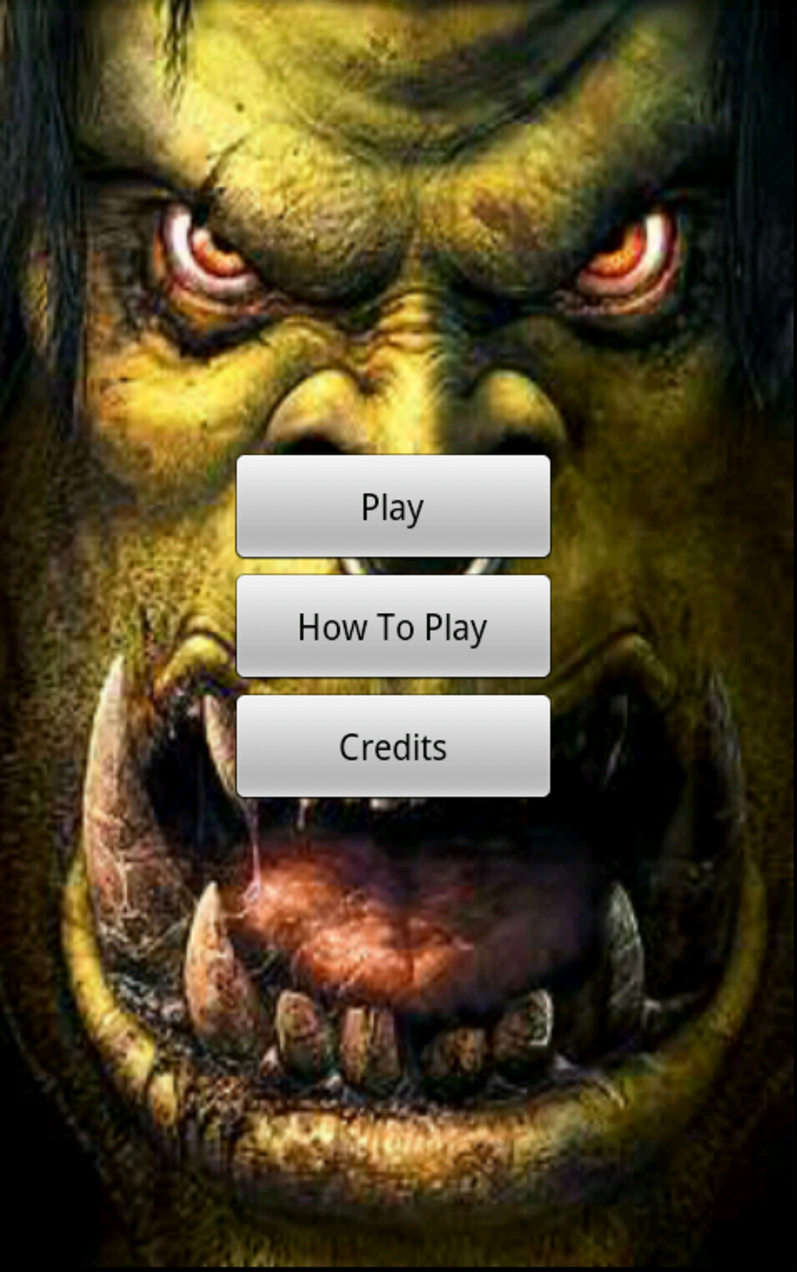
\includegraphics[scale=0.5]{main/figures/screenshots/menu}
		\caption{Main Menu}
		\label{usermanual:menu}
\end{figure}

The options you have when in the main menu is:

\begin{itemize}
	\item Play -- pressing this button will start the game
	\item How To Play -- If you press this button you will get a fast tutorial on how to play the game.
	\item Credits -- The credits will be displayed
\end{itemize}



\subsection{The Game}
You have pressed the “Play” button, and the game have now started. The first wave will after a little while start to appear, and you shall kill it by building towers.

The mobs will be walking on a brown dirt road, while the empty green fields can be used for tower building. Figure \ref{usermanual:startGame} shows how the start of the game looks like.

\begin{figure} [h]
	\center
		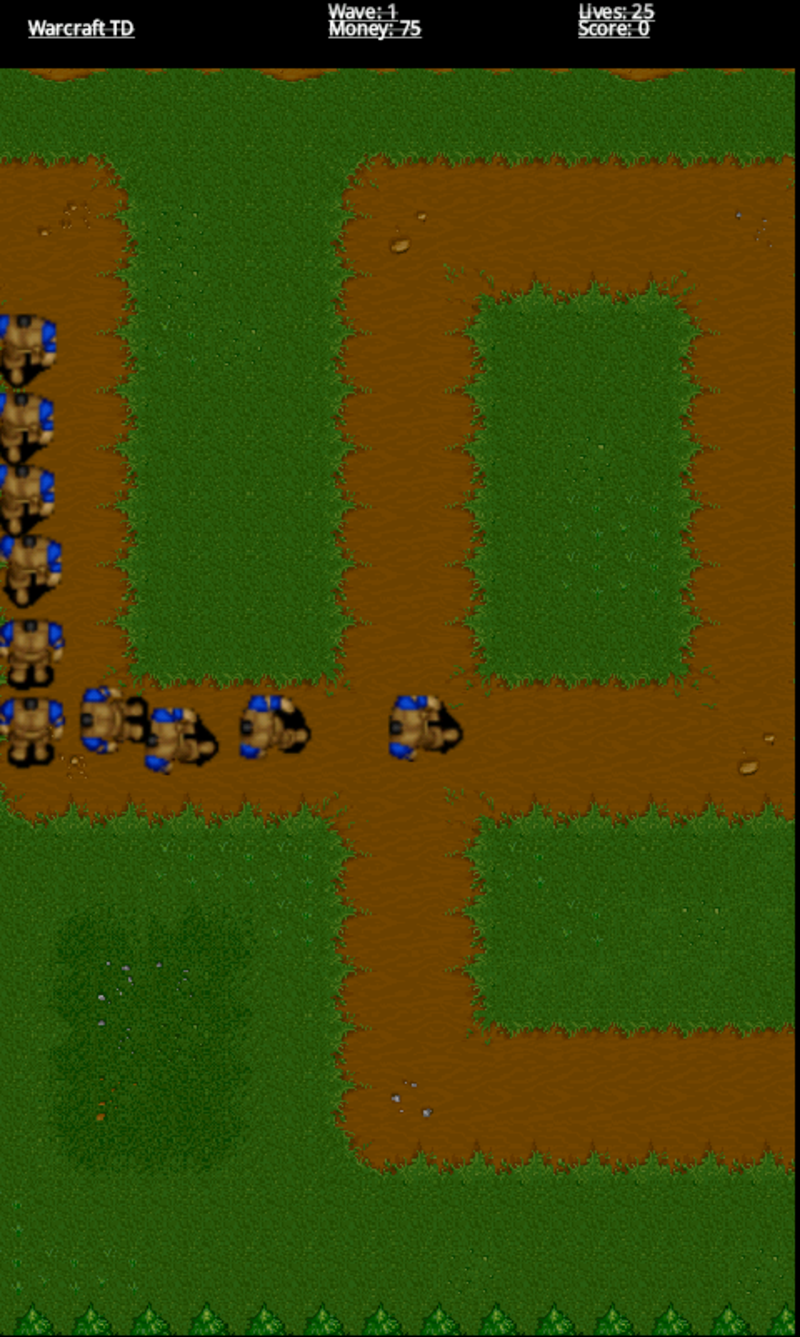
\includegraphics[scale=0.5]{main/figures/screenshots/play}
		\caption{Start of game}
		\label{usermanual:startGame}
\end{figure}

\subsection{Building Towers}
When the game has started you can start building your first tower. To get the Tower Menu to appear, you need to press the spot you want to build a tower, and hold for one second. When the Tower Menu appears, you choose which tower to build by clicking the chosen tower. If you don’t have enough resources for a special tower, that tower will be grayed out in the dialog. Figure \ref{usermanual:createTower} shows how the dialog looks like.

\begin{figure} [h] 
	\center
		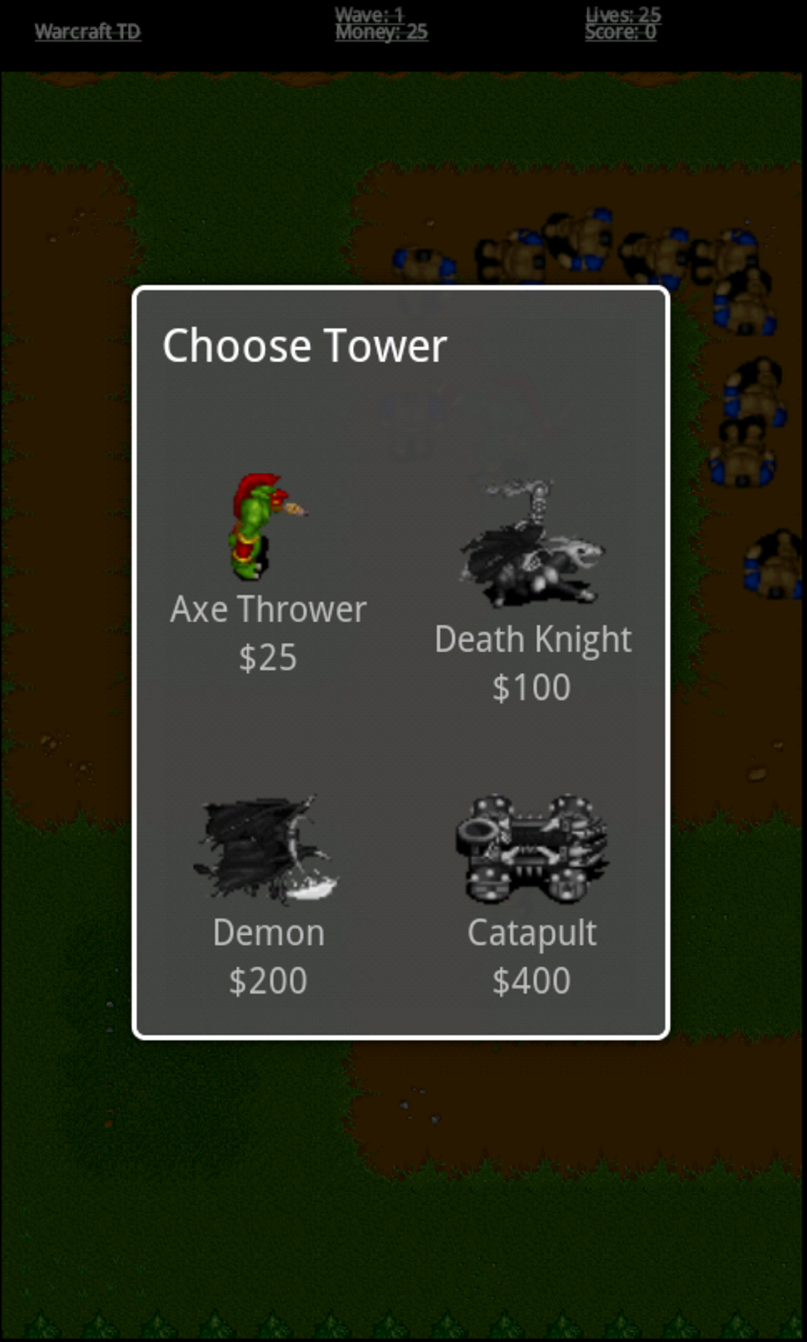
\includegraphics[scale=0.5]{main/figures/screenshots/create_tower}
		\caption{Create Tower Dialog}
		\label{usermanual:createTower}
\end{figure}

There are four different types of towers. The towers have increasing range and damage, aswell as price. 

\begin{itemize}
	\item Axe Thrower: A tower dealing minor damage
	\item Death Knight: A tower dealing medium damage
	\item Demon: A tower dealing high damage 
	\item Catapult: A tower dealing massive damage
\end{itemize}

Towers should be placed in key positions where they can shoot enemies for the longest time. It is up to the player to decide which positions will give the best results. Figure \ref{usermanual:gameplay} displays the game after placing a couple of towers.
\clearpage
\begin{figure} [h]
	\center
		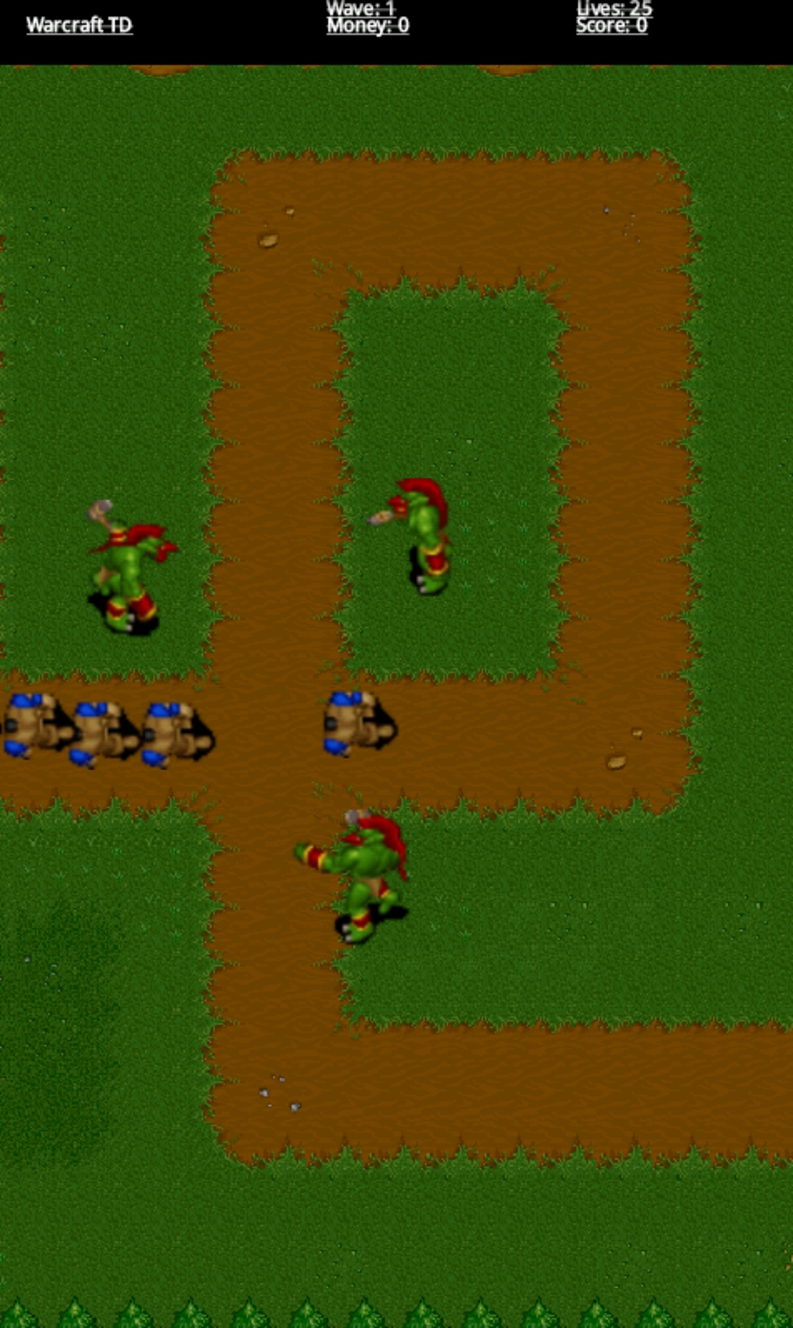
\includegraphics[scale=0.5]{main/figures/screenshots/gameplay}
		\caption{Gameplay}
		\label{usermanual:gameplay}
\end{figure}

%\subsection{Developer Guide}

%Here follows a short introduction on how to the application can be modified.

%All changes to the game has to be done before compilation time. We have tried to make it relatively easy to make changes or additions to the game or its content.

%\subsubsection{Creating a new map}
